\clearpage
\setcounter{page}{1}
\maketitlesupplementary

\begin{strip}
  \vspace{-0em}
  \centering
  \captionsetup{type=table} %suppresses caption warning

\renewcommand{\arraystretch}{1.1}
\setlength{\tabcolsep}{4.5pt}
\centering
\renewcommand{\arraystretch}{1.1}
\setlength{\tabcolsep}{4pt}
\begin{tabular}{llccccccccc}
\toprule
Method & Metric & \texttt{chess} & \texttt{fire} & \texttt{heads} & \texttt{office} & \texttt{pumpkin} & \texttt{redkitchen} & \texttt{stairs} & Avg \\
\midrule
\multirow{4}{*}{CUT3R}
& Accuracy     & 0.274 & 0.102 & 0.106 & 0.326 & 0.452 & 0.325 & 0.345 & 0.276 \\
& Completeness & 0.303 & 0.081 & 0.093 & 0.441 & 0.459 & 0.358 & 0.389 & 0.303 \\
& Chamfer      & 0.289 & 0.091 & 0.100 & 0.384 & 0.456 & 0.342 & 0.367 & 0.290 \\
& ATE   & 0.743 & 0.226 & 0.363 & 0.664 & 0.546 & 0.381 & 0.413 & 0.477 \\
\midrule
\multirow{4}{*}{SLAM3R}
& Accuracy     & 0.043 & 0.022 & 0.020 & 0.035 & 0.072 & 0.062 & 0.116 & 0.053 \\
& Completeness & 0.030 & 0.013 & 0.015 & 0.030 & 0.055 & 0.061 & 0.209 & \underline{0.059} \\
& Chamfer      & 0.037 & 0.018 & 0.017 & 0.033 & 0.064 & 0.061 & 0.162 & \underline{0.056} \\
& ATE   & 0.089 & 0.048 & 0.036 & 0.088 & 0.196 & 0.102 & 0.126 & 0.098 \\
\midrule
\multirow{4}{*}{MASt3R-SLAM}
& Accuracy     & 0.090 & 0.037 & 0.027 & 0.047 & 0.097 & 0.070 & 0.045 & 0.059 \\
& Completeness & 0.055 & 0.024 & 0.021 & 0.053 & 0.054 & 0.036 & 0.149 & \bf{0.056} \\
& Chamfer      & 0.073 & 0.031 & 0.024 & 0.050 & 0.075 & 0.053 & 0.097 & 0.057 \\
& ATE   & 0.063 & 0.046 & 0.029 & 0.103 & 0.112 & 0.074 & 0.032 & \underline{0.066} \\
\midrule
\multirow{4}{*}{VGGT-SLAM}
& Accuracy     & 0.029 & 0.014 & 0.031 & 0.041 & 0.128 & 0.036 & 0.087 & \underline{0.052} \\
& Completeness & 0.052 & 0.064 & 0.021 & 0.066 & 0.054 & 0.057 & 0.110 & 0.061 \\
& Chamfer      & 0.040 & 0.039 & 0.026 & 0.054 & 0.091 & 0.047 & 0.098 & \underline{0.056} \\
& ATE   & 0.037 & 0.026 & 0.022 & 0.103 & 0.147 & 0.063 & 0.095 & 0.070 \\
\midrule
\multirow{4}{*}{Ours}
& Accuracy     & 0.065 & 0.015 & 0.031 & 0.036 & 0.061 & 0.035 & 0.074 & \bf{0.045} \\
& Completeness & 0.063 & 0.022 & 0.040 & 0.048 & 0.037 & 0.030 & 0.154 & \bf{0.056} \\
& Chamfer      & 0.064 & 0.019 & 0.035 & 0.042 & 0.049 & 0.033 & 0.114 & \bf{0.051} \\
& ATE   & 0.073 & 0.035 & 0.028 & 0.055 & 0.129 & 0.035 & 0.029 & \bf 0.055 \\
\bottomrule
\end{tabular}
\vspace{7pt}
\caption{\textbf{Per Scene Evaluation on 7-Scenes~\cite{shotton2013-7scenes}.} Comparison of accuracy, completeness, Chamfer distance, and trajectory error on the 7-Scenes dataset. Lower is better. Best results are \textbf{bold}, second best are \underline{underlined}.}
\label{tab:7scenes_results_full}
\vspace{4em}
\end{strip}






\section{Relative Scale in Pose Graph}
As mentioned in \cref{subsec:backend}, the \textit{scale edges} connect nodes corresponding to the same view but obtained from different forwarding passes. Since the training supervision of the frontend STA model uses only normalized pointmaps, the scales of the same view across different passes are not consistent. Therefore, estimating the relative scale is crucial for pose graph construction.
Given two pointmaps $\bm{P}_i^j$ and $\bm{P}_i^k$ of the same view $i$ (obtained from forwarding passes with input view $i\  j$ and view $i\ k$, respectively), along with their confidence maps $\bm{C}_i^j$ and $\bm{C}_i^k$, we first get the confidence score $w_{x}$ of the point pair for pixel $\bm x$,
\begin{align}
    w_{x} = &\bm C_i^j(\bm x) \cdot \bm C_i^k(\bm x), \nonumber
\end{align}
then, the relative scale $s_i^{jk}$ can be computed as,
\begin{align}
    s_i^{jk} =& \min_s \sum_{\bm x} w_{x}\| \bm P_i^j(\bm x)-s\bm P_i^k(\bm x) \|^2 \nonumber \\
    =& \dfrac{\sum_{\bm x}w_{x}(\bm P_i^j(\bm x)\cdot \bm P_i^k(\bm x))}{\sum_{\bm x}w_{x}\|\bm P_i^k(\bm x)\|^2}.
\end{align}



\section{Additional Quantitative Results}

\subsection{Per Scene Evaluation Results on 7-Scenes}
In \cref{subsec:recon}, only the average reconstruction evaluation is provided. In \cref{tab:7scenes_results_full}, we present more detailed per-scene results on 7-Scenes~\cite{shotton2013-7scenes} to offer deeper insights. The pure regression method SLAM3R~\cite{liu2025slam3r} performs well in scenes where the camera primarily focuses on a single corner, such as \texttt{chess}, \texttt{fire}, and \texttt{heads}. However, in scenes involving longer camera trajectories, like \texttt{pumpkin} and \texttt{redkitchen}, its performance degrades due to difficulties in accurately registering points. Our method, \ours, achieves the best performance in average across all four metrics.

\subsection{Additional Trajectory Results on TUM-RGBD}
In \cref{subsec:traj}, to align with previous methods, only results for the \textit{freiburg1} partition of the TUM RGB-D dataset~\cite{sturm12tumrgbd} are reported. In \cref{tab:traj_tumrgbd_more}, we also report results for the \textit{freiburg2} and \textit{freiburg3} partitions.

\begin{table}[h]
    \centering
    \begin{tabular}{l c}
        \toprule
        \textbf{Sequence} & \textbf{ATE RMSE (m)} \\
        \midrule
        freiburg2\_360\_hemisphere        & 0.2037 \\
        freiburg2\_360\_kidnap            & 0.4617 \\
        freiburg2\_desk                   & 0.0577 \\
        freiburg2\_large\_with\_loop      & 0.2170 \\
        freiburg2\_rpy                    & 0.0222 \\
        freiburg2\_xyz                    & 0.0155 \\
        \midrule
        freiburg3\_cabinet                & 0.3869 \\
        freiburg3\_large\_cabinet         & 0.1334 \\
        freiburg3\_long\_office\_household & 0.1013 \\
        freiburg3\_teddy                  & 0.0789 \\
        \bottomrule
    \end{tabular}
    \caption{\bf Trajectory ATE results on the \textit{freiburg2} and \textit{freiburg3} partitions of the TUM RGB-D dataset~\cite{sturm12tumrgbd}.}
        \label{tab:traj_tumrgbd_more}
\end{table}




\subsection{Additional Evaluation on More Datasets}
In \cref{tab:replica_eval} and \cref{tab:scannet_eval}, we additionally report camera trajectory evaluation results on Replica~\cite{replica19arxiv} and ScanNet~\cite{dai2017scannet}, as well as reconstruction evaluation results on Replica for several commonly used SLAM testing scenes.


\begin{table}[h]
    \centering
    \begin{tabular}{l c c c c}
        \toprule
        \textbf{Scene} & \textbf{ATE} & \textbf{Acc.} & \textbf{Comp.} & \textbf{Chamfer} \\
        \midrule
        office0 & 0.0744 & 0.0595 & 0.0226 & 0.0410 \\
        office1 & 0.1934 & 0.2614 & 0.1833 & 0.2223 \\
        office2 & 0.1177 & 0.0914 & 0.0316 & 0.0615 \\
        office3 & 0.0485 & 0.0623 & 0.0221 & 0.0422 \\
        office4 & 0.1302 & 0.1338 & 0.0688 & 0.1013 \\
        room0   & 0.0688 & 0.0766 & 0.0209 & 0.0488 \\
        room1   & 0.0934 & 0.1105 & 0.0552 & 0.0828 \\
        room2   & 0.1363 & 0.1194 & 0.0223 & 0.0709 \\
        \bottomrule
    \end{tabular}
    \caption{\bf Per-scene evaluation results on Replica~\cite{replica19arxiv}.}
    \label{tab:replica_eval}
    \vspace{1.5em}
% \end{table}


% \begin{table}[h]
\setlength{\tabcolsep}{25pt}
    \centering
    \begin{tabular}{l c}
        \toprule
        \textbf{Sequence} & \textbf{ATE RMSE (m)} \\
        \midrule
        scene0000\_00 & 0.0483 \\
        scene0059\_00 & 0.0391 \\
        scene0106\_00 & 0.0559 \\
        scene0169\_00 & 0.0526 \\
        scene0181\_00 & 0.0520 \\
        scene0207\_00 & 0.0479 \\
        \bottomrule
    \end{tabular}
    \caption{\bf Per-scene camera trajectory evaluation results on ScanNet~\cite{dai2017scannet}.}
        \label{tab:scannet_eval}
\end{table}


\begin{figure*}[!htb]
\centering
{\small
    \setlength{\tabcolsep}{15pt}
    \renewcommand{\arraystretch}{1}
    \newcommand{\sz}{0.4}
    \begin{tabular}{cc}
      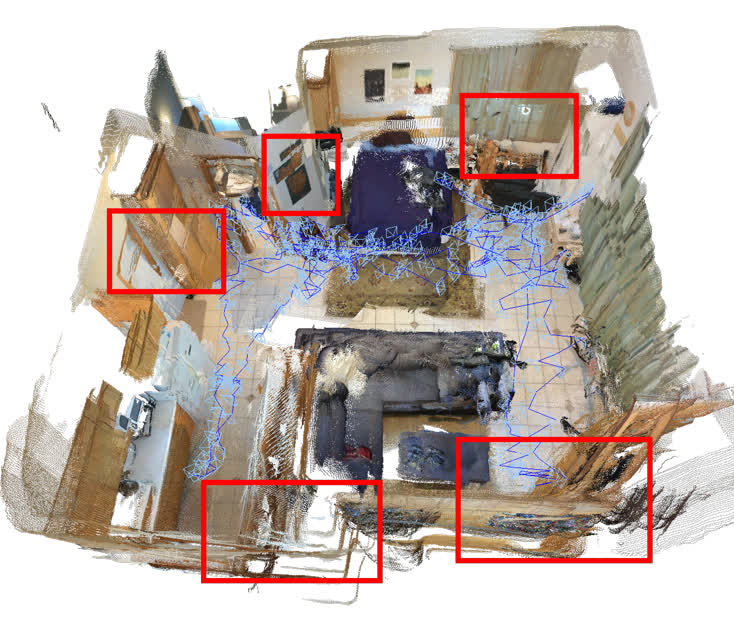
\includegraphics[width=\sz\linewidth]{figs/supp/scannet00_nopgo.jpg} &
      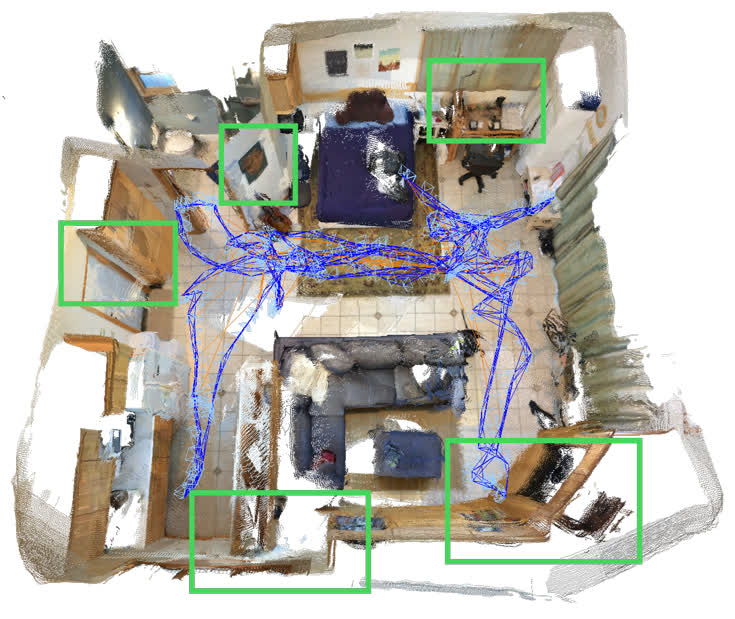
\includegraphics[width=\sz\linewidth]{figs/supp/scannet00.jpg} \\
      result \wo PGO & result \emph{w/} PGO

    \end{tabular}
}
\vspace{7pt}
\caption{\textbf{Qualitative Comparison for Pose Graph Optimization.} Red boxes highlight regions with misalignments, while green boxes indicate areas where these misalignments have been corrected after pose graph optimization.
}
\label{fig:pgo}
\vspace{2.5em}

\centering
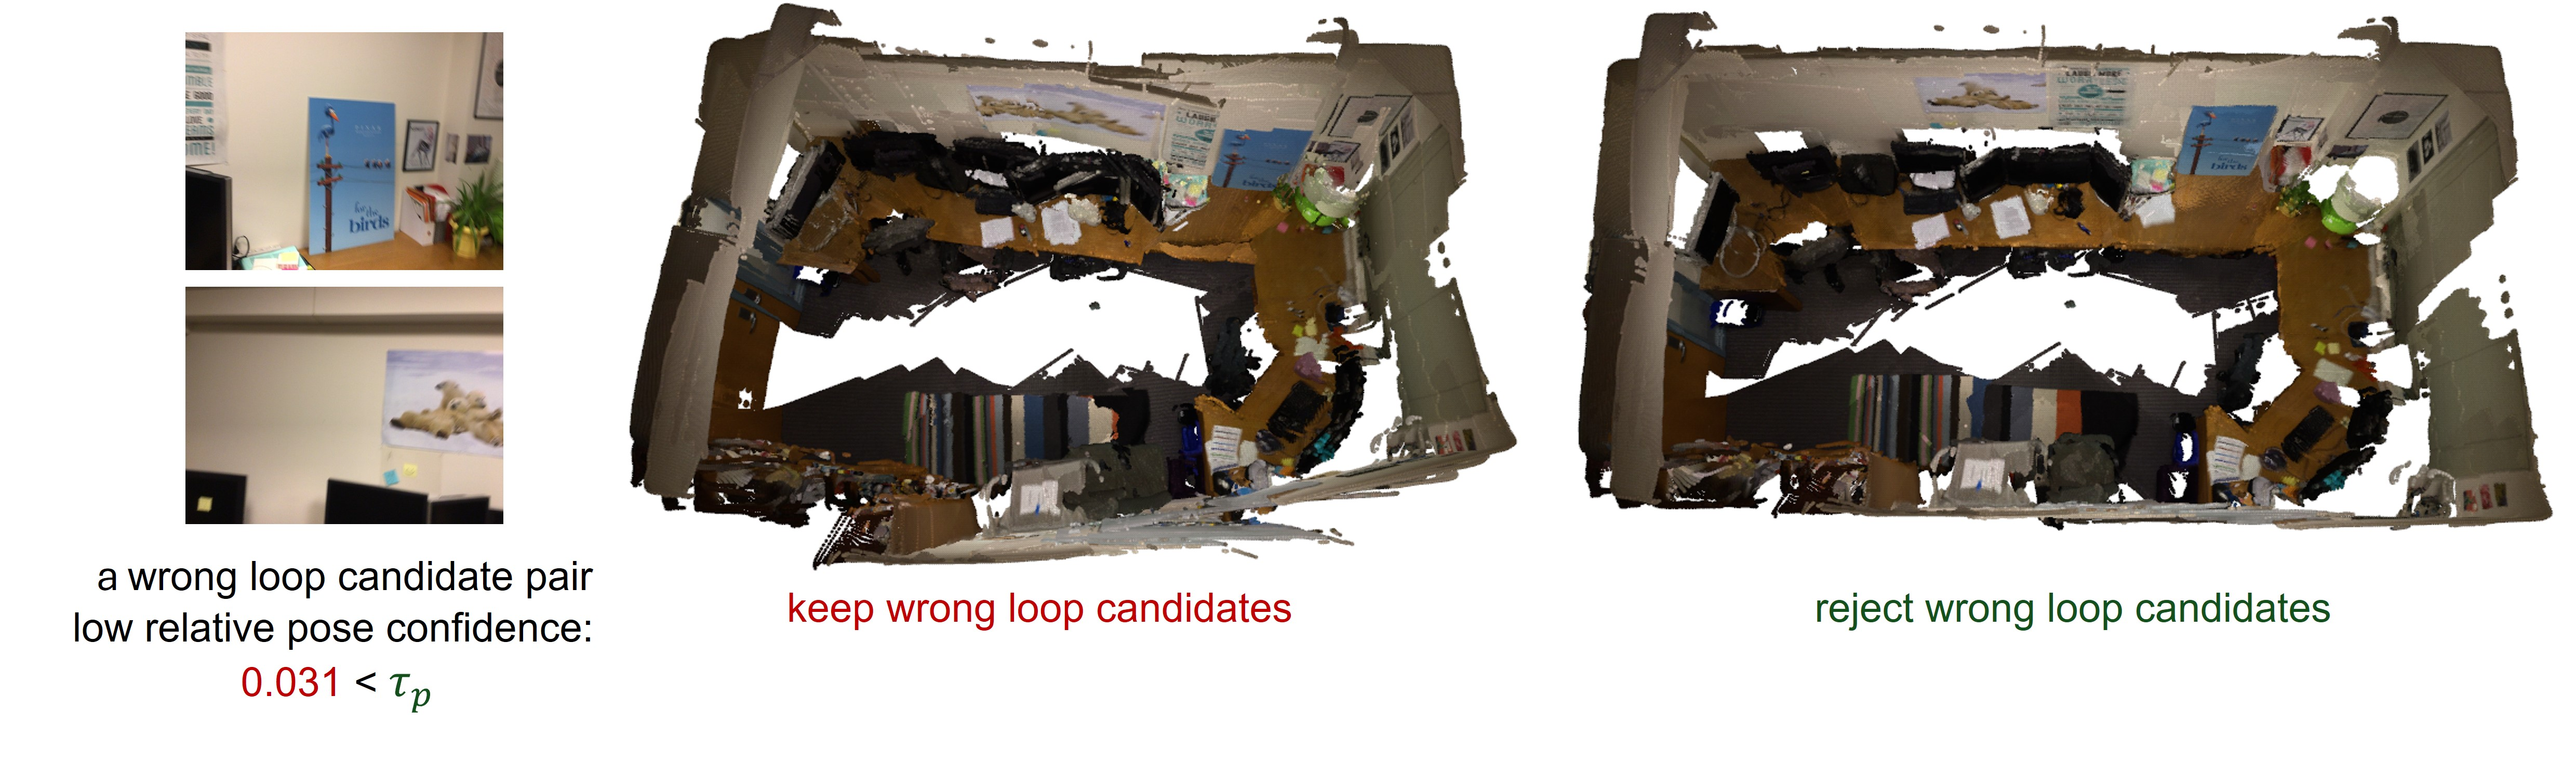
\includegraphics[width=\linewidth]{figs/supp/wrong_loop.jpg}
\vspace{-1.7em}
\caption{\textbf{Qualitative Comparison of Wrong Loop Filtering.} Keeping wrong loop candidates decreases the performance a lot.}
\label{fig:wrong_loop}

\end{figure*}

\section{Additional Qualitative Results}




\subsection{Pose Graph Optimization}
In \cref{fig:pgo}, we compare the reconstruction and trajectory estimation results with and without pose graph optimization on ScanNet~\cite{dai2017scannet} \texttt{scene0000\_00}. Pose graph optimization effectively corrects misaligned areas and averages out the errors from the frontend.

\subsection{Wrong Loop Filtering}
In \cref{subsec:backend}, we describe feeding each loop candidate pair into our STA model to verify their spatial proximity. This is necessary because Bag of Words loop detection can produce false positives, which may significantly degrade performance by introducing misleading edges into the pose graph. As shown in \cref{fig:wrong_loop}, rejecting incorrect loop candidates using the relative pose confidence score provided by STA results in a much more stable performance.


\subsection{More Results}
In \cref{fig:more}, we present the results of \ours across various datasets. \ours demonstrates stable performance despite differing camera motions in these scenes. As before, light blue frustums represent camera poses, blue lines connect neighboring views, while orange lines indicate loop closures.




\begin{figure*}[!htb]
\centering
{\small
    \setlength{\tabcolsep}{25pt}
    \renewcommand{\arraystretch}{1}
    \newcommand{\sz}{0.38}
    \begin{tabular}{cc}
      BundleFusion~\cite{dai2017bundlefusion} \texttt{apt2} & TUM-RGBD~\cite{sturm12tumrgbd} \texttt{floor} \\
      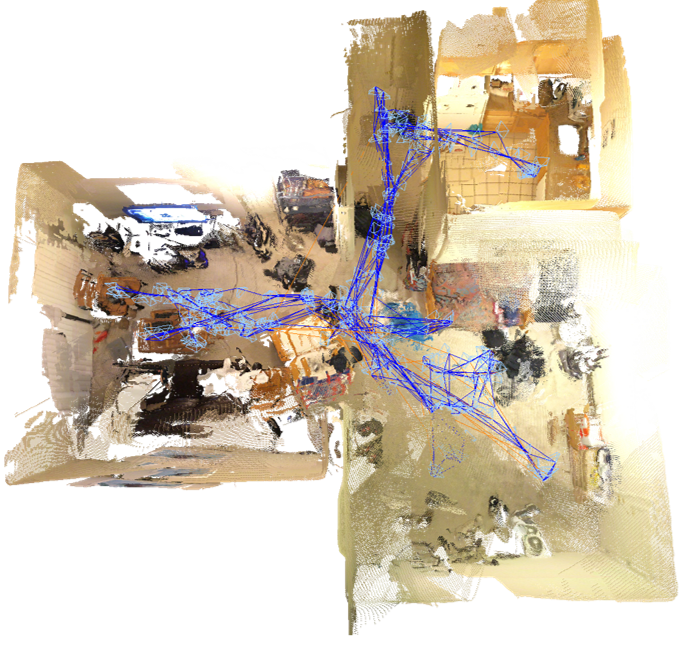
\includegraphics[width=\sz\linewidth]{figs/supp/bf_apt2.png} &
      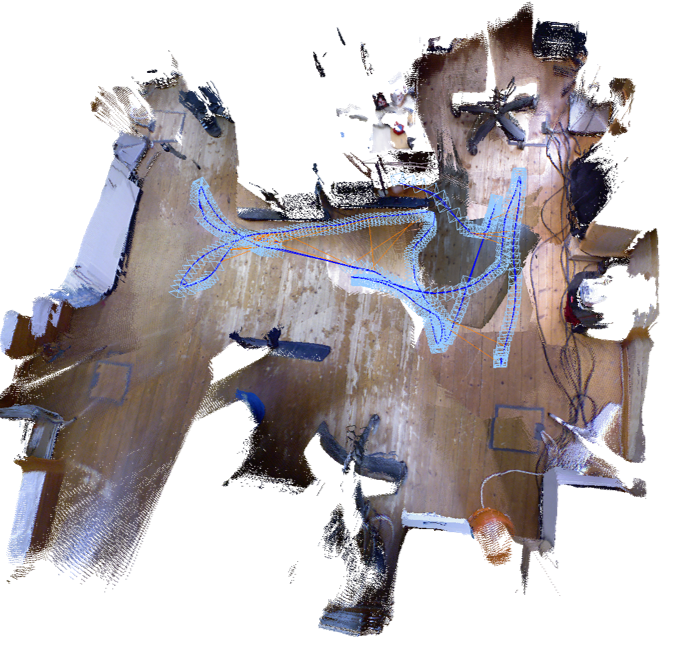
\includegraphics[width=\sz\linewidth]{figs/supp/tum_floor.png} \\

      BundleFusion~\cite{dai2017bundlefusion} \texttt{apt0} & 7-Scenes~\cite{shotton2013-7scenes} \texttt{pumpkin}  \\
      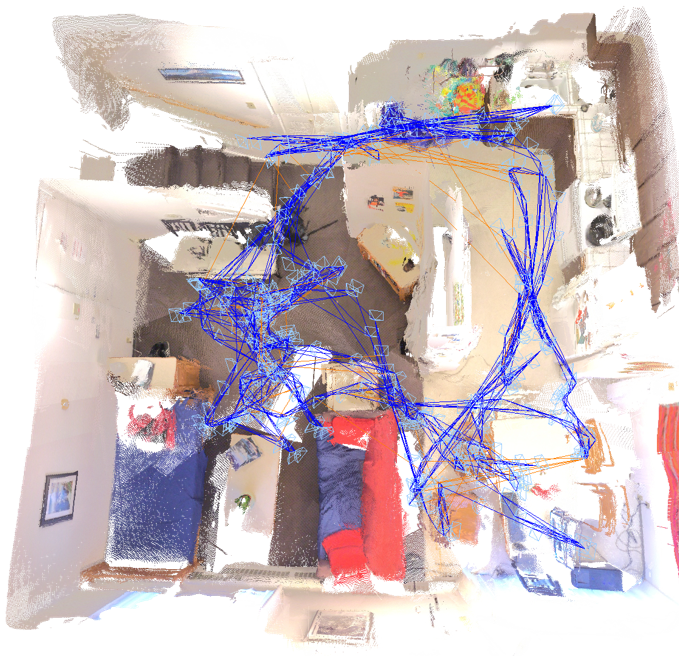
\includegraphics[width=\sz\linewidth]{figs/supp/bf_apt0.png} &
      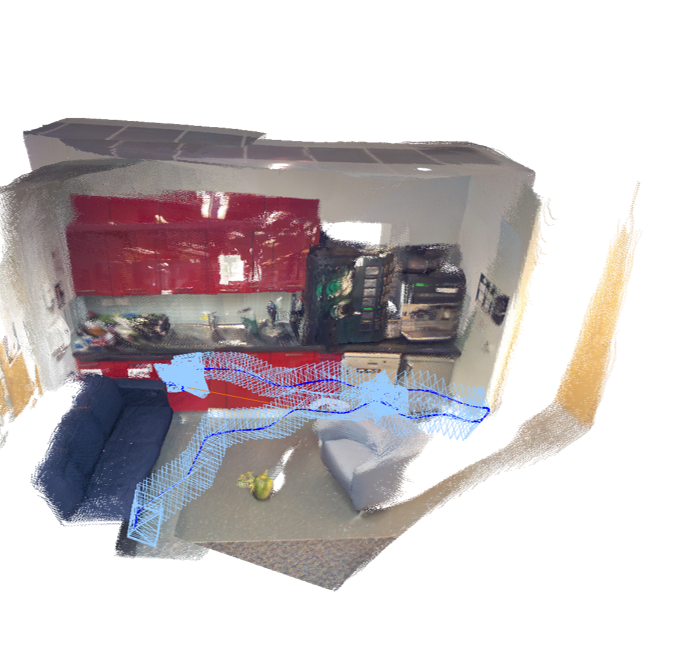
\includegraphics[width=\sz\linewidth]{figs/supp/7scenes_redkitchen.png} \\

      M2DGR~\cite{yin2021m2dgr} \texttt{room\_03} & M2DGR~\cite{yin2021m2dgr} \texttt{room\_01}  \\
      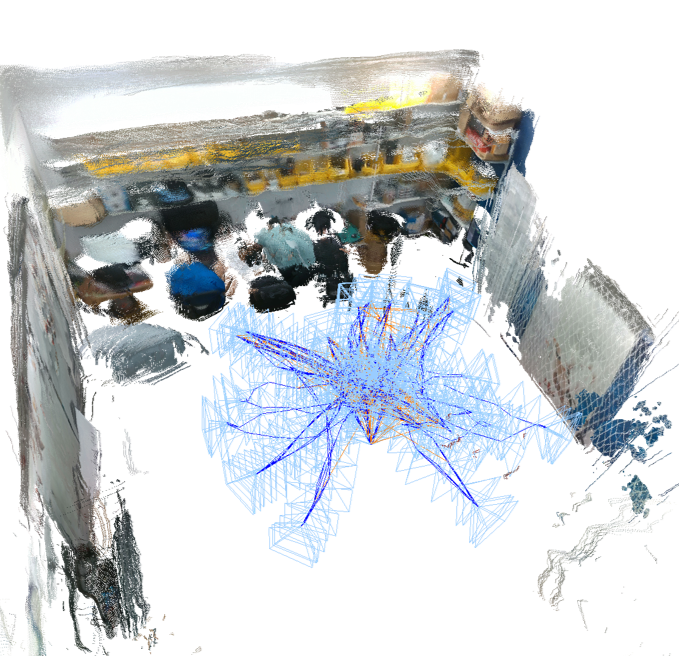
\includegraphics[width=\sz\linewidth]{figs/supp/m2dgr_room03.png} &
      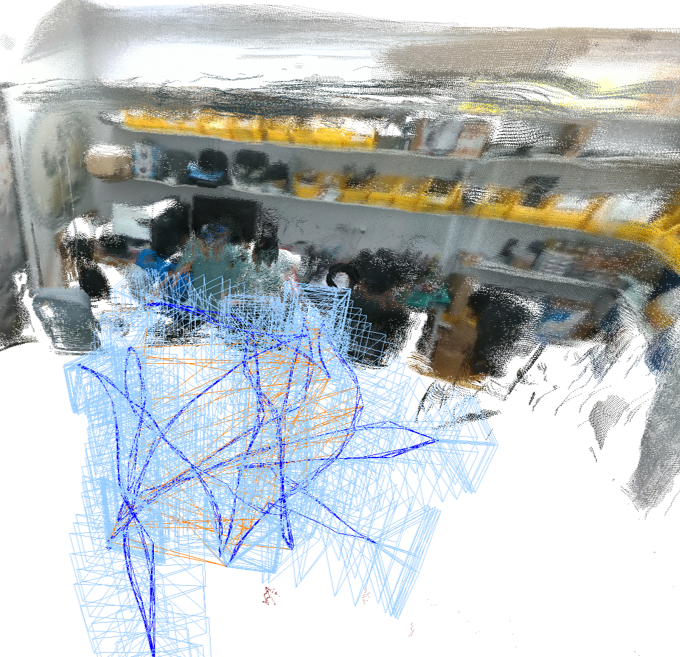
\includegraphics[width=\sz\linewidth]{figs/supp/m2dgr_room01.png} \\
    \end{tabular}
}
% \vspace{8pt}
\caption{\textbf{More Qualitative Results.} Reconstructions and camera trajectories from different datasets.}
\label{fig:more}
\end{figure*}


% \section{Rationale}
% \label{sec:rationale}
% %
% Having the supplementary compiled together with the main paper means that:
% %
% \begin{itemize}
% \item The supplementary can back-reference sections of the main paper, for example, we can refer to \cref{sec:intro};
% \item The main paper can forward reference sub-sections within the supplementary explicitly (e.g. referring to a particular experiment);
% \item When submitted to arXiv, the supplementary will already included at the end of the paper.
% \end{itemize}
% %
% To split the supplementary pages from the main paper, you can use \href{https://support.apple.com/en-ca/guide/preview/prvw11793/mac#:~:text=Delete%20a%20page%20from%20a,or%20choose%20Edit%20%3E%20Delete).}{Preview (on macOS)}, \href{https://www.adobe.com/acrobat/how-to/delete-pages-from-pdf.html#:~:text=Choose%20%E2%80%9CTools%E2%80%9D%20%3E%20%E2%80%9COrganize,or%20pages%20from%20the%20file.}{Adobe Acrobat} (on all OSs), as well as \href{https://superuser.com/questions/517986/is-it-possible-to-delete-some-pages-of-a-pdf-document}{command line tools}.
